\documentclass[11pt,a4paper]{article}
\usepackage[utf8]{inputenc}
\usepackage[T1]{fontenc}
\usepackage[english]{babel}
\usepackage[english]{isodate}
\usepackage[paper=a4paper]{geometry}
\newgeometry{top=3.5cm,bottom=2.5cm,right=2.5cm,left=2.5cm}
\usepackage{graphicx}
\usepackage{comment}
\usepackage{fancyhdr}
\usepackage{framed}
\usepackage{lastpage}
\usepackage[hidelinks]{hyperref}
\usepackage{tabularx}
\usepackage[table]{xcolor}
\usepackage{enumitem}
\usepackage{mdwlist}
\usepackage{placeins}
\usepackage{amsmath}
\usepackage{xcolor}
\usepackage{listings}
\usepackage{amssymb}
\usepackage{lmodern}
\usepackage{array, tabularx}
\renewcommand{\tabularxcolumn}[1]{>{\raggedright}m{#1}}
\newcolumntype{Y}{ >{\hsize =0.8\hsize}X}
\newcolumntype{Z}{ >{\hsize =1.2\hsize}X}
\usepackage{makecell}
\renewcommand\theadfont{\bfseries}
\renewcommand\theadalign{lc}
\renewcommand\cellalign{lc}
\usepackage{cellspace}
\setlength\cellspacetoplimit{5pt}
\setlength\cellspacebottomlimit{5pt}
\addparagraphcolumntypes{X, Y, Z}
\usepackage{algorithm}
\usepackage[noend]{algpseudocode}



\begin{document}

%%%%%%%%%%%%%%%%%%%%%%%%%%%%%%%%%%%%%%%%%%%%%%%%%%%%%%%%%%%%%%%%%%%%%%%%%%%%%%%%
% DEFINIZIONI
%%%%%%%%%%%%%%%%%%%%%%%%%%%%%%%%%%%%%%%%%%%%%%%%%%%%%%%%%%%%%%%%%%%%%%%%%%%%%%%%

\newcommand{\titolo}  {Assignment 2}
\newcommand{\nome}    {SpamFilter}
\newcommand{\versione}{2.0}

%%%%%%%%%%%%%%%%%%%%%%%%%%%%%%%%%%%%%%%%%%%%%%%%%%%%%%%%%%%%%%%%%%%%%%%%%%%%%%%%
%% SETUP DOCUMENTO
%%%%%%%%%%%%%%%%%%%%%%%%%%%%%%%%%%%%%%%%%%%%%%%%%%%%%%%%%%%%%%%%%%%%%%%%%%%%%%%%

%%%%%%%%%%%%%%%%%%%%%%%%%%%%%%%%%%%%%%%%%%%%%%%%%%%%%%%%%%%%%%%%%%%%%%%%%%%%%%%%
% TITOLO
%%%%%%%%%%%%%%%%%%%%%%%%%%%%%%%%%%%%%%%%%%%%%%%%%%%%%%%%%%%%%%%%%%%%%%%%%%%%%%%%
\newcommand{\image}[3]{ % 1 image 2 caption 3 size
	\begin{figure}[h!]
		\centering
		\includegraphics[width=#3\textwidth]{#1} 
		\caption{#2}
	\end{figure}
	\FloatBarrier
}

\newcommand{\R}{{\rm I\!R}}

\newcommand{\imageLabel}[4]{ % 1 image 2 caption 3 size
	\begin{figure}[h!]
		\centering
		\includegraphics[width=#3\textwidth]{#1} 
		\caption{#2}
		\label{fig:#4}
	\end{figure}
	\FloatBarrier
}
\newcommand{\Z}{\mathbb{Z}}

\pagenumbering{Alph}
\begin{titlepage}
	\begin{center}
		
\includegraphics[width=0.7\textwidth]{unive}
		
		\vspace*{1cm}
		\LARGE
		\textit{Artificial Intelligence: knowledge representation and planning\\ \center Year: 2017/2018}
		
		\vspace{0.5cm}
		\Huge
		\textbf{\titolo}\\
		\LARGE {\nome}
		
		\line(1,0){280}
		
		\vspace{0.5cm}
		\large
		

		\Large
		\Large Author: \textbf{Antonio Emanuele Cinà} \\
		\vspace{0.5cm}

		\textit{\today }
		
		\vfill
		
	\end{center}
\end{titlepage}

%%%%%%%%%%%%%%%%%%%%%%%%%%%%%%%%%%%%%%%%%%%%%%%%%%%%%%%%%%%%%%%%%%%%%%%%%%%%%%%%
%% STILE HEADER - FOOTER - LISTE
%%%%%%%%%%%%%%%%%%%%%%%%%%%%%%%%%%%%%%%%%%%%%%%%%%%%%%%%%%%%%%%%%%%%%%%%%%%%%%%%

\renewcommand{\headheight}{14pt}

\pagestyle{fancy}
\lhead{}
\chead{}
\lhead{\textit{Author: acina}}
\rhead{\textbf{\titolo}}
\cfoot{}
\renewcommand{\headrulewidth}{0.4pt}
\renewcommand{\footrulewidth}{0.4pt}

%\renewcommand{\labelitemi}{$\diamond$}
%\renewcommand{\labelitemii}{$\bullet$}
\renewcommand{\labelitemi}{$\bullet$}
\renewcommand{\labelitemii}{$\diamond$}
\renewcommand{\labelitemiii}{$\circ$}

\setlist{itemsep=0pt}

\setlength{\parindent}{0cm}

%%%%%%%%%%%%%%%%%%%%%%%%%%%%%%%%%%%%%%%%%%%%%%%%%%%%%%%%%%%%%%%%%%%%%%%%%%%%%%%%
%% INDICE
%%%%%%%%%%%%%%%%%%%%%%%%%%%%%%%%%%%%%%%%%%%%%%%%%%%%%%%%%%%%%%%%%%%%%%%%%%%%%%%%

\pagenumbering{gobble}
\renewcommand{\contentsname}{Index}
\tableofcontents
\newpage
\pagenumbering{arabic}

%%%%%%%%%%%%%%%%%%%%%%%%%%%%%%%%%%%%%%%%%%%%%%%%%%%%%%%%%%%%%%%%%%%%%%%%%%%%%%%%
%% FOOTER CON NUMERO PAGINA
%%%%%%%%%%%%%%%%%%%%%%%%%%%%%%%%%%%%%%%%%%%%%%%%%%%%%%%%%%%%%%%%%%%%%%%%%%%%%%%%

\rfoot{\thepage\ di \pageref{LastPage}}



\definecolor{mygreen}{rgb}{0,0.6,0}
\definecolor{mygray}{rgb}{0.5,0.5,0.5}
\definecolor{mymauve}{rgb}{0.58,0,0.82}

\lstset{ %
	backgroundcolor=\color{white},   % choose the background color; you must add \usepackage{color} or \usepackage{xcolor}; should come as last argument
	basicstyle=\footnotesize,        % the size of the fonts that are used for the code
	breakatwhitespace=false,         % sets if automatic breaks should only happen at whitespace
	breaklines=true,                 % sets automatic line breaking
	captionpos=b,                    % sets the caption-position to bottom
	commentstyle=\color{mygreen},    % comment style
	deletekeywords={...},            % if you want to delete keywords from the given language
	escapeinside={\%*}{*)},          % if you want to add LaTeX within your code
	extendedchars=true,              % lets you use non-ASCII characters; for 8-bits encodings only, does not work with UTF-8
	frame=single,	                   % adds a frame around the code
	keepspaces=true,                 % keeps spaces in text, useful for keeping indentation of code (possibly needs columns=flexible)
	keywordstyle=\color{blue},       % keyword style
	language=Octave,                 % the language of the code
	morekeywords={*,...},            % if you want to add more keywords to the set
	numbers=left,                    % where to put the line-numbers; possible values are (none, left, right)
	numbersep=5pt,                   % how far the line-numbers are from the code
	numberstyle=\tiny\color{mygray}, % the style that is used for the line-numbers
	rulecolor=\color{black},         % if not set, the frame-color may be changed on line-breaks within not-black text (e.g. comments (green here))
	showspaces=false,                % show spaces everywhere adding particular underscores; it overrides 'showstringspaces'
	showstringspaces=false,          % underline spaces within strings only
	showtabs=false,                  % show tabs within strings adding particular underscores
	stepnumber=2,                    % the step between two line-numbers. If it's 1, each line will be numbered
	stringstyle=\color{mymauve},     % string literal style
	tabsize=2,	                   % sets default tabsize to 2 spaces
	title=\lstname                   % show the filename of files included with \lstinputlisting; also try caption instead of title
}

\lstset{
	language=Python,
	basicstyle=\ttfamily,
	otherkeywords={self},             
	keywordstyle=\ttfamily\color{blue!90!black},
	keywords=[2]{True,False,reshape},
	keywords=[3]{ttkc},
	keywordstyle={[2]\ttfamily\color{orange}},
	keywordstyle={[3]\ttfamily\color{red!80!orange}},
	emph={MyClass,__init__, False, True,dot,reshape,SVC,cross_val_score},          
	emphstyle=\ttfamily\color{red!80!black},    
	stringstyle=\color{cyan!80!black},
	showstringspaces=false            
}


%\begin{table}[!htbp]
%	\begin{tabularx}{\linewidth}{|Y|l|l|S{Z}|l}
%		\cline{1-4}
%		\thead{Risk Event} & \thead{Chance\\ of Happening} & \thead{Severity} & \thead{Measures\\ to be taken} & \\
%		\cline{1-4}
%		Team member\break missing meetings & Significant & Low & Encourage team members to read over minutes and inform of any tasks set. If regularly absent issue a warning and then card. & \\
%		\cline{1-4}
%		QA/Project manager missing meetings & Significant & Low/Moderate & Deputy in role will act as manager. & \\
%		\cline{1-4}
%		Team member leaving project group & Low & Moderate/High & List all tasks assigned to missing team member and reassign them, after this refactor the timetable and planning. & \\
%		\cline{1-4}
%	\end{tabularx}%
%\end{table}

%%%%%%%%%%%%%%%%%%%%%%%%%%%%%%%%%%%%%%%%%%%%%%%%%%%%%%%%%%%%%%%%%%%%%%%%%%%%%%%%
%% SEZIONI
%%%%%%%%%%%%%%%%%%%%%%%%%%%%%%%%%%%%%%%%%%%%%%%%%%%%%%%%%%%%%%%%%%%%%%%%%%%%%%%%

\section {Introduction}
Write a spam filter using \textbf{discriminative} and \textbf{generative} classifiers. Use the Spambase dataset which already represents spam/ham messages through a bag-of-words representations through a dictionary of 48 highly discriminative words and 6 characters. The first 54 features correspond to word/symbols frequencies; ignore features 55-57; feature 58 is the class label (1 spam/0 ham).
\begin{itemize}
	\item Perform SVM classification using linear, polynomial of degree 2, and RBF kernels over the TF-IDF representation. Can you transform the kernels to make use of angular information only (i.e., no length)? Are they still positive definite kernels?
	
	\item Classify the same data also through a Naive Bayes classifier for continuous inputs, modeling each feature with a Gaussian distribution, resulting in the following model:
	
	$$p(y = k) = \alpha_k$$
	$$p(x| y = k) = \prod_{i = 1}^{D} \left[ (2\pi\sigma_{ki}^2)^{-\frac{1}{2}} \exp\left\{-\frac{1}{2\sigma_{ki}^2(x_i - \mu_{ki})^2}\right\}\right]$$
\end{itemize}
where $\alpha_k$ is the frequency of class $k$, and $\mu_{ki}$, $\sigma^2_{ki}$ are the means and variances of feature $i$ given that the data is in class $k$. \\
Provide the code, the models on the training set, and the respective performances in 10 way cross validation. Explain the differences between the two models.\\

\section{Classification problem}
In machine learning and statistics one of the most common problem is represented by \textbf{classification}. Starting from input data observation (\textbf{feature vectors}) a classification algorithm uses them in order to learn a model which is able in the future to assign \textbf{labels} to new observations. The labels considered for this assignment are essentially two $0,1$ representing if a message is ham or spam. For example given a dataset of email labeled with 0 (ham) and 1 (spam), a classification problem consists on learning a model that will assign as better as possible the label predicted for the new email, not previously seen during the learning phase. \\
Formally speaking let $X = (X_1, ..., X_m) \in \mathcal{X}$ as the predictors of our problem and let $Y \in \mathcal{Y} $ the target variable which specify the class of the observations. The classification problem consists on learning a function $\phi: \mathcal{X} \rightarrow \mathcal{Y}$ from a \textit{training set}.
Considering the task of this assignment we can define $\mathcal{Y} = \{0,1\}$ so that:
$$\phi(x) = g(f(x))$$
where $f(x)$ is a discrimination function which ideally separate objects of class $0$ from objects of class $1$, and $g(z)$ with $z = f(x)$ is a function that returns the right label to assign to the new message $x$ according to the result of $f(x)$. Essentially in our case $g(x)$ is so defined:  
$$
g(z)=
\begin{cases}
1\qquad \text{the message is spam} \qquad \text{if} \quad z \geq \varepsilon\\
0\qquad \text{otherwise the message is ham}\\
\end{cases}
$$
Where $\varepsilon$ is a decision threshold that is learned during learning phase.

\section{Discriminative and Generative classifiers}
In general there are three kinds of learning algorithms: supervised, unsupervised and reinforcement learning.\\
\textbf{Supervised learning} is a formalization of the idea of learning from example observations. A supervised algorithms takes in input a set of observations $X$ and its labels $Y$, and learns a model considering the pairs $(x_i, y_i)$.
\textbf{Unsupervised learning} algorithms try to learn a model for prediction starting from unlabeled data. The last one, \textbf{reinforcement learning}, is not supported directly by training data points, but there is an agent that interact with the environment, making observations or taking actions, and it is rewarded or punished. The goal of the agent is to learn the way to be rewarded.\\
The problem of this assignment belongs to the class of supervised learning approaches, so during the following document we will focus our attention to them.
In general a classifiers can be defined as: \textbf{Generative} or \textbf{Discriminative}.
Before introducing the two models first it is necessary to give some probability notions:
\begin{itemize}
	\item $p(x)$, is the probability of observing $x$ from its domain space.
	\item $p(y)$, is the probability of the class $y$.
	\item $p(y|x)$, we can read this probability like "the probability that the given observed value $x$ belongs to the class $y$". It is the condition probability and it represents the probability of assigning the class $y$ to the given observation $x$.
	\item $p(x|y)$, is the so called \textbf{prior probability} and it can be described as the probability of generating/observing $x$ from the class $y$.
\end{itemize}
Discriminative classifiers model the posterior probability $p(y|x)$ directly, or learn a direct map from inputs $x$ to the labels $y$.
Generative classifiers learn a model of the joint probability $p(x,y)$ of the inputs $x$ and the label $y$ and make their predictions by using Bayes rules to calculate $p(y|x)$ and then pick the most likely label $y$. Generative classifiers try to learn the join probability distribution $p(x,y)$ using the prior probability $p(x|y)$ and the class probability $p(y)$.

\section{Support Vector Machine}
The first model that we are going to analyze is the \textbf{Support Vector Machine} (SVM) classifier. It belongs to the class of discriminative classifiers since its goal consists on learning the class boundary between the two classes $y$ starting from features $x$. In order to simplify the notation we will substituted the original labeling $y= \{0,1\}$ with a new one $y= \{-1,1\}$.
We can formally define the SVM linear classifier in this way:
$$h_{w,b}(x) = g(w^Tx + b)$$
$$
g(z)=
\begin{cases}
1\qquad \text{if} \quad z \geq 0\\
-1\qquad \text{otherwise}\\
\end{cases}
$$
Where $w^T + b$ represents a \textbf{separating hyperplane} for the two classes, and $g(z)$ is the decision function which returns the predicted class for the observation $x$. \\
We define the probability of classification given an observation $x$ as:
$$p(y = 1 | x; w,b)$$
In our problem the classifier would then predict $1$ (spam) if $h_{w,b}(x) \geq 0$, which is equivalent of considering $w^Tx + b \geq 0$, and $-1$ (ham) otherwise.\\
We can also say that the larger $w^Tx + b$ is, the higher is the confidence that the label is $1$. \\

This result is a consequence of the fact that if $w^Tx + b$ increase then also $h_{w,b}(x)= p(y = 1 | x; w,b)$ becomes larger. The same thing is valid with label $-1$, in this case we would like to have $w^Tx + b$ as small as possible $w^Tx + b \ll 0$.\\

\begin{figure}[!h]
	\begin{minipage}[t]{0.5\linewidth}
		\centering
		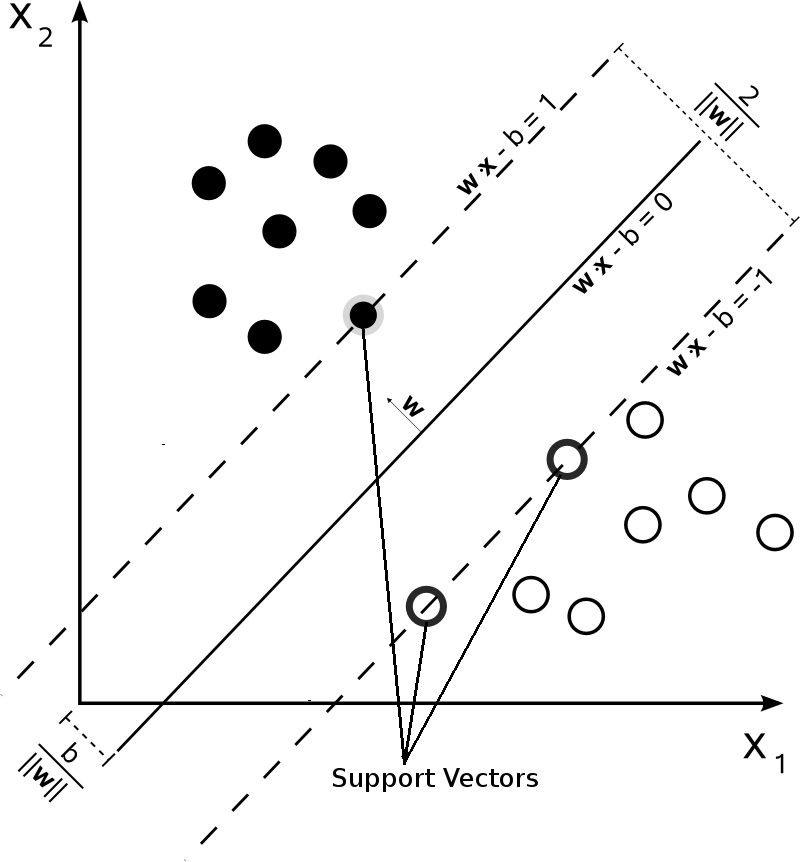
\includegraphics[width=0.8\textwidth]{img/SVMPlot2.png}
		\caption{Support Vector Machines classifier}
		\label{f1}
	\end{minipage}
	\hspace{0.1cm}
	\begin{minipage}[t]{0.5\linewidth} 
		\centering
		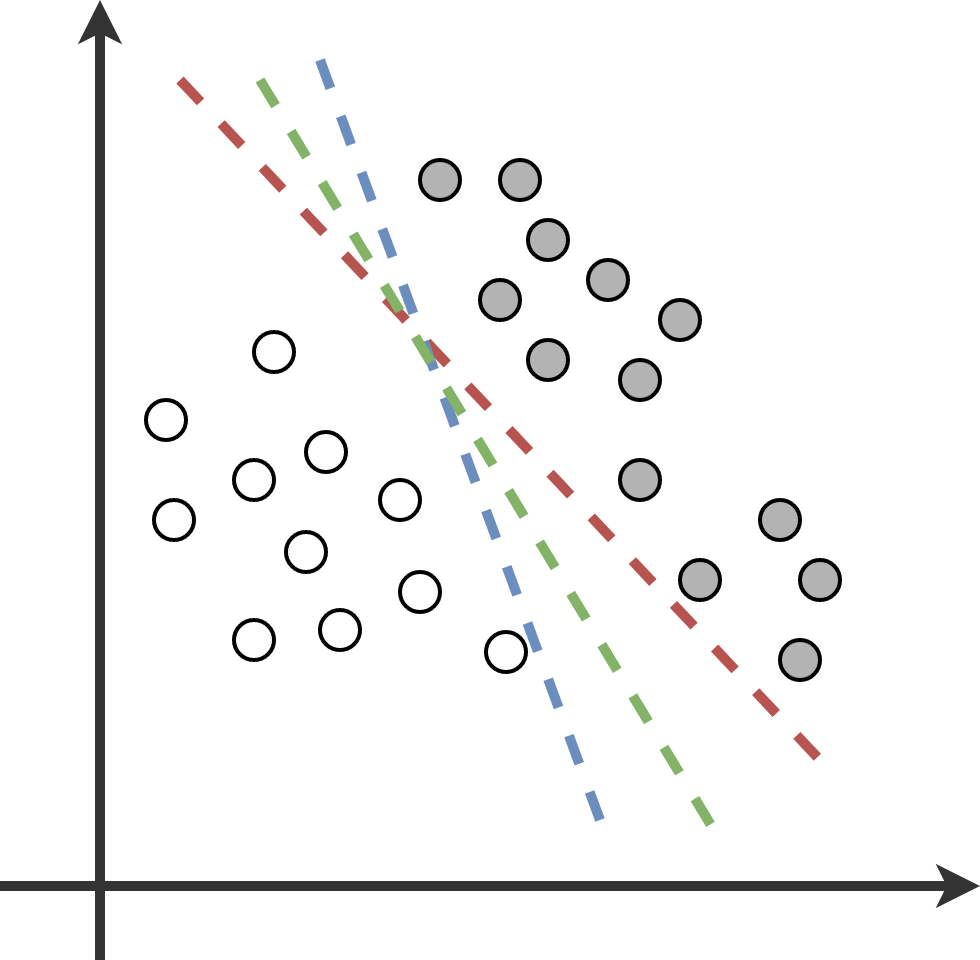
\includegraphics[width=0.9\textwidth]{img/separating-lines.png}
		\caption{Possible separating hyperplanes}
		\label{f2}
	\end{minipage}        
\end{figure} 

Figure 1 shows an application of a SVM classifier. In this example we have two classes $1$ and $-1$ represented in a $2$ dimensional space using respectively filled points and empty ones. The line given by the equation $w^Tx + b = 0$ defines the separate hyperplane which works as a \textbf{decision boundary} of our problem. But Figure 2 introduce a problem which must be considered: Which is the right hyperplane? In general it is possible to find an infinite number of hyperplane that separate the two classes, but they can produce different results, performance and also can have effects on the robustness of the classifier.\\
Before going in details of the best hyperplane it is necessary to introduce the following concepts: \textbf{functional margin} and \textbf{geometric margin}.

\paragraph{Functional margin} it is a testing that function verify if a particular point is properly classified or not.
$$\hat{\gamma}^{(i)} = y^{(i)}(w^Tx^{(i)} + b)$$
When $\hat{\gamma}^{(i)} > 0$ the prediction of the observation $i$ is correct, and the larger is the functional margin result the greater is the confidence of the current prediction. However it cannot be considered as a very good measure of confidence since it is affected by the length of the two vectors $w, b$. In fact, considering the pair $(\alpha w, \alpha b)$ we can notice that the new functional margin if multiplied by the factor $\alpha$. For that reason could be reasonable to set $||w||_2 = 1$, but we will discuss about it later.
% TODO RIVEDERE L'ULTIMA FRASE

\paragraph{Geometric margin} it represents the euclidean distance between a point and the decision boundary.
\image{img/geometricMargin.png}{Geometric margin}{0.45}
Considering the previous figure, $A$ is a point representing the $i$ observation and $B$ is a point on the straight line defined by $w^TB+b = 0$. We can so define the geometrical margin $\gamma^{(i)}$ as the length of the segment $AB$. \\

Now that we have defined the notion of geometric and functional margin it is possible to give an idea of which is the best hyperplane. This concept, as we are going to see, is strictly related to the two margins. We define the \textbf{geometric margin} $\gamma$ and the \textbf{functional margin} $\hat{\gamma}$ respect to the training set $S = \{(x^{(i)},y^{(i)}); i = 1,\dots,m \}$ the following value:
$$\gamma = \underset{i = 1,\dots,m}{\text{min }}\gamma^{(i)}$$
$$\hat{\gamma} = \underset{i = 1,\dots,m}{\text{min }}\hat{\gamma}^{(i)}$$


This values $\gamma$ represents the distance from the decision boundary to the closest point. An interesting property of the geometric margin is that it is related with the functional margin by the following definition: $\gamma = \frac{\hat{\gamma}}{||w||}$. \\
The idea of an SVM classifier is to find a separating hyperplane which maximizes the geometric margin. The resulting hyperplane is so considered as the best one since it separates better then other ones the two classes.\\
Formally speaking the main goal of Support Vector Machine is to solve the following optimization problem:

\begin{equation*}
\begin{aligned}
&\text{max }_{\gamma,w,b} \quad \gamma\\
&\text{s.t.} \quad y^{(i)}(w^Tx^{(i)}+b) \geq \gamma \qquad i = 1,\dots, m\\
&||w|| = 1
\end{aligned}
\end{equation*}
The constraint $||w|| = 1$, that we have seen previously, is now introduced to enforce that the functional margin is equal to the geometric one, so that the problem can be rewritten as:
\begin{equation*}
\begin{aligned}
&\text{max }_{\hat{\gamma},w,b} \quad \frac{\hat{\gamma}}{||w||}\\
&\text{s.t.} \quad y^{(i)}(w^Tx^{(i)}+b) \geq \hat{\gamma} \qquad i = 1,\dots, m\\
\end{aligned}
\end{equation*}
\newpage

Now the non-convex constraint $||w|| = 1$ is introduced directly inside the target function and instead of considering the geometric margin the optimization problem is re-formulated in terms of functional margin. Now imposing the scaling constraint $\hat{\gamma}$ = 1 it is possible to rewrite the same optimization problem as a minimization of $||w||^2$:
\begin{equation*}
 \begin{aligned}
 &\text{min }_{\gamma,w,b} \quad \frac{1}{2}||w||^2\\
 &\text{s.t.} \quad y^{(i)}(w^Tx^{(i)}+b) \geq 1 \qquad i = 1,\dots, m\\
 \end{aligned}
\end{equation*}
This formulation represent an optimization problem on a convex function and with only linear constraints. Its solution is an \textbf{optimal margin classifier}. The points with the minimum margin from the decision boundary are called \textbf{support vectors}. The advantage of SVM is that instead of considering all the possible points SV from the training set it considers only these points to determine the decision boundary. Using the \textbf{Lagrange} function with $m$ Lagrange multipliers $(\lambda_1,\dots,\lambda_m)$ it is possible to rewrite the correspondent optimization problem, with parameters $w$ and $b$, into an identical one but with parameters $(\lambda_1,\dots,\lambda_m)$. Taking advantage of the dual representation we can write the new optimization problem as follow:
\begin{equation*}
\begin{aligned}
&\text{max }\quad L_D(\lambda_1,\dots,\lambda_m) = \sum_{i = 1}^{m}\lambda_i - \frac{1}{2}\sum_{i = 1}^{m}\sum_{j = 1}^{m}\lambda_i\lambda_jy_iy_jx_i^Tx_j\\
&\text{s.t.} \quad \sum_{i = 1}^{m}\lambda_iy_i= 0 \qquad \lambda_i \geq 0, \forall i = 1,\dots,m\\
\end{aligned}
\end{equation*}
Note that the training vectors appears only as dot products, and the advantage of using this formulation is that only support vectors will be the only Lagrange multipliers such that $\lambda_i > 0$, and the others are essentially equal to zero (sparse solution). Now the maximum margin hyperplane is given by:
$$\sum_{i = 1}^{m} y_i \lambda_ix_i^Tx+b = 0$$


Until now we worked with the assumption that the space is linearly separable, but SVM allows a strategy called \textbf{kernel trick} for learning a possible separating hyperplane in a new space.
In some cases could be interesting or evaluating not the original space but a transformation of it, for instance when in the original space data points are not linearly separable. We define a function $\phi(x)$ as the function that applies a mapping of a feature vector to another one. The SVM algorithm now instead of considering the vector $x$ learns using the resulting vector of $\phi(x)$. A \textbf{kernel} function is nothing else that an inner product between feature mappings of $\phi$:
$$K(x,z) = \phi(x)^T\phi(z)$$
Informally speaking a kernel function is a similarity measure between the feature mapping $x$ and $z$. 
The advantage of using this technique is that it allows to learn in the high dimensional feature space of a transformation of it defining a function $\phi$. Since the SVM algorithm works with only inner products between input vectors ($x$,$z$), then we can replace the simple inner product with a kernel function in order to learns in a different feature space that in some cases could be more efficient. But there is a restriction on the function $K$, it must satisfy the following property in order to be considered a \textbf{valid kernel}:
$$K(x,z) = \phi(x)^T\phi(z) \qquad \forall x, z \in S$$
\newpage
Another interesting property is the positivity of a kernel:
\paragraph{Definition} 
A symmetric function  $K: \mathbb{R}^n\times\mathbb{R}^n \rightarrow \mathbb{R}$ is said to be \textbf{positive definite kernel} if:
$$\sum_{i=1}^n \sum_{j=1}^n c_i c_j K(x_i, x_j) \geq 0	\qquad c_i,c_j \in \mathbb{R}$$

In the following assignment we are going to deal with the following positive definite kernels:
\begin{itemize}
	\item \textbf{Linear}: $K(x_i,x_j) = x_i^Tx_j$
	\item \textbf{Polynomial of degree 2}: $K(x_i,x_j) = (1 + x_i^Tx_j)^2$
	\item \textbf{Gaussian Radial Basis Function} (RBF): 
	$K(x_i, x_j) = \exp\left(-\frac{\|x_i - x_j\|^2}{2\sigma^2}\right)$
\end{itemize}
\begin{figure}[!h]
	\begin{minipage}[t]{0.5\linewidth}
		\centering
		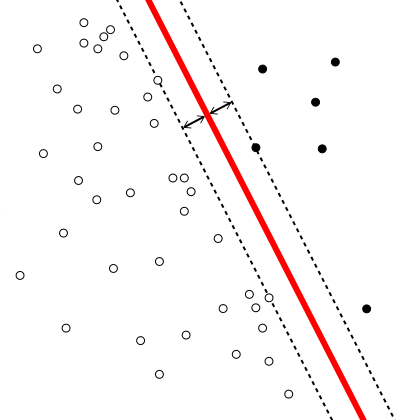
\includegraphics[width=0.61\textwidth]{img/Linear_Kernel_Machine.png}
		\caption{SVM: Linear Kernel}
		\label{f1}
	\end{minipage}
	\hspace{0.1cm}
	\begin{minipage}[t]{0.5\linewidth} 
		\centering
		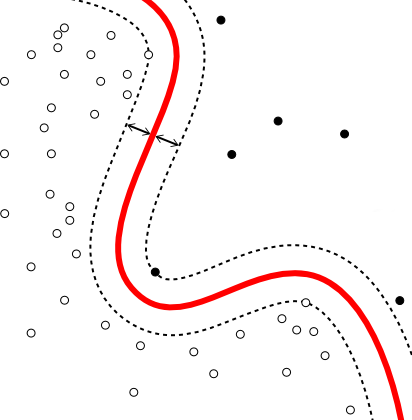
\includegraphics[width=0.61\textwidth]{img/Poly_Kernel_Machine.png}
		\caption{SVM: Polynomial Kernel}
		\label{f2}
	\end{minipage}        
\end{figure} 
\image{img/RBF_Kernel.png}{SVM: Radial Basis Function Kernel}{0.4}

\subsection{Angular kernels}
One of the goal for this assignment is to build new kernels that use angular information only. The kernels defined until now (linear, polynomial and Gaussian RBF) are affected by the length of each vector, so that two vectors with the same direction (angle) but with different length results not so similar. Now if we want to consider only the direction of each vector is necessary to normalize vector such that at the end $||x||_2 = 1$. We know that a kernel is defined as:
$$\phi: \mathbb{R}^m \rightarrow \mathbb{R}^m \qquad \phi(x) = \frac{x}{||x||}$$
$$K(x_i,x_j) = \phi(x_i)^T\phi(x_j)= \frac{x_i}{||x_i||} \frac{x_j}{||x_j||} = \cos(x_i,x_j)$$
We can see that this kernel is not affected by the length of the two vector but it only considers the \textit{cosine} of the angle create by two vectors $x_i$, $x_j$.\\

So we have seen that it is possible to consider only angular information, but another consideration must be done: Are they still positive definite kernels?
In order to answer to this question it is necessary to prove that:
 
$$\sum_{i=1}^n \sum_{j=1}^n c_i c_j K(x_i, x_j) \geq 0	\qquad c_i,c_j \in \mathbb{R}$$

\begin{equation*}
\begin{split}
&\quad\sum_{i = 1}^{n}\sum_{j=1}^{n}c_ic_jK(x_i,x_j) \qquad \text{n number of points}\\
&=\sum_{i = 1}^{n}\sum_{j=1}^{n}c_ic_j\langle\phi(x_i),\phi(x_j)\rangle \\
&=\sum_{i=1}^{n}\sum_{j=1}^{n}c_ic_j\sum_{k=1}^{m}\frac{x_{ik}}{||x_{ik}||}\frac{x_{jk}}{||x_{jk}||} \qquad \text{m number of features} \\
&=\sum_{i=1}^{n}\sum_{j=1}^{n}\sum_{k=1}^{m}c_i\frac{x_{ik}}{||x_{ik}||}c_j\frac{x_{jk}}{||x_{jk}||} \\
&=\sum_{k=1}^{m}\Big(\sum_{i=1}^{n}c_i\frac{x_{ik}}{||x_{ik}||}\Big)\Big(\sum_{j=1}^{n}c_j\frac{x_{jk}}{||x_{jk}||}\Big)\\
&=\sum_{k=1}^{m}\Big(\sum_{i=1}^{n}c_i\frac{x_{ik}}{||x_{ik}||}\Big)^2 \geq 0\\
\end{split}
\end{equation*}

Regarding the other two kernels, radial basis and polynomial of degree 2, we can write their kernel in this way:
$$K_{p}(x_i,x_j) = \phi_p(x_i)^T\phi_p(x_j) $$
$$K_{rb}(x_i,x_j) = \phi_{rb}(x_i)^T\phi_{rb}(x_j) $$
From the theory we know that these kernels are positive definite. Now if we are interested on applying the two kernels but considering only the angular information, and not the length of vectors, we can modify the feature mapping in this way:
$$\phi_{p}^\prime(x) = \phi_{p}\Big(\frac{x}{||x||}\Big) \qquad \qquad \phi_{bf}^\prime(x) = \phi_{bf}\Big(\frac{x}{||x||}\Big)$$

$$K_{p}^\prime(x_i,x_j) =  \phi_{p}^\prime(x_i)^T\phi_{p}^\prime(x_j) = \phi_{p}\Big(\frac{x_i}{||x_i||}\Big)^T\phi_{p}\Big(\frac{x_j}{||x_j||}\Big) = K_{p}\Big(\frac{x_i}{||x_i||},\frac{x_j}{||x_j||}\Big)\geq 0$$

$$K_{bf}^\prime(x_i,x_j) =  \phi_{bf}^\prime(x_i)^T\phi_{bf}^\prime(x_j) = \phi_{bf}\Big(\frac{x_i}{||x_i||}\Big)^T\phi_{bf}\Big(\frac{x_j}{||x_j||}\Big) = K_{bf}\Big(\frac{x_i}{||x_i||},\frac{x_j}{||x_j||}\Big)\geq 0$$

Since $K_{p}$ and $K_{bf}$ are positive definite kernel so the property is satisfied also for the two new kernels: $K_{p}^\prime$, $K_{bf}^\prime$. With these proves we have seen that the three new kernel, that are not affected by length of the vectors, are valid positive definite kernels.


\subsection{Implementation and Results}
For this assignment I decided to use the python library \textbf{sklearn}, which is an open source tool for data mining and analysis. The SVM classifier is already developed and provided by the library. But before applying the SVM classifier, it is necessary to apply the \textbf{TF-IDF transformation} of the original dataset, that measures the relevance of a term respect to term frequency inside the document and its presence on the other documents in the collection.
$$\text{score}(i,j) = tf_{i,j}\times idf_i$$
$$idf_i = \ln \frac{|D|}{|d: i \in d|}$$

Where:
\begin{itemize}
	\item $\text{score}(i,j)$ is the score of the term $i$ inside the document $j$.
	\item $tf_{i,j}$ is the frequency of the term $i$ in the document $j$.
	\item $idf_i$ is the inverse document frequency of the term $i$ which measures its relevance.
	\item $D$ collection of documents.
\end{itemize}
%TODO: scrivere del tf-idf dei caratteri
Now using the library sklearn it is easily to implement the SVM classifiers with the three kernels:
\begin{lstlisting}[language=Python]
Y = email[0:,57] # classes
X = tfidf(email[:,:54]) # values
clf = SVC(kernel="linear", C = 1.0)
clf_poly = SVC(kernel="poly", degree = 2,C = 1.0)
clf_rbf = SVC(kernel="rbf", C = 1.0)
\end{lstlisting}
Note the presence of the argument \textbf{C}, which controls the influence of each individual support vector. Large values of C give solutions with less misclassification errors but a smaller margin, instead small values of C give solutions with bigger margin and more classification errors. In other words if C is small we are generalizing maybe too much, if it is larger probably we are overfitting the model.  Tuning the parameter C is not the goal of this assignment but should be considered in real application, since it can give very different results.\\

Performance of the resulting model are retrieved using \textbf{10-way Cross-validation}. Cross-validation is an iterative technique to evaluate predictive models by splitting at each iteration the original dataset into a training set, used to train the model, and a test set, used to measure the goodness of the model. K-Way Cross-validation consists on splitting the total dataset in K parts, at iteration $j$ the $j-th$ part is used for testing and the others are user for training. This technique avoids \textbf{overfitting}, in which the model learns also noise coming from the training set, and asymmetric sampling of dataset. In case of overfitting the model learns too well the training set but later is not able to generalize and predict well new data. Instead asymmetric sampling can introduce bias on the model given by the structure or composition of data inside the training set.
Also in this case the library sklearn provides an easy way to perform cross-validation using multi-cores:

\begin{lstlisting}[language=Python]
scores = cross_val_score(clf, X, Y, cv = 10, n_jobs= 8)
print("Min accuracy Linear Kernel: " + str(scores.min()))
print("Mean accuracy Linear Kernel: " + str(scores.mean()))
print("Max accuracy Linear Kernel: " + str(scores.max()))
\end{lstlisting}
The following table summarize the results obtained using the three different kernels, that use also length of vectors:
\begin{table}[!htbp]
	\begin{tabularx}{\linewidth}{|Y|l|l|l|l|}
		\cline{1-5}
		\centering{\textbf{Kernel}} & \thead{Min score} & \thead{Mean score} & \thead{Max score} &  \thead{Deviance} \\
		\cline{1-5}
		\centering \textit{Linear} & $0.6034$ & $0.6079$ & $0.6174$ &   $0.00358$\\
		\cline{1-5}
		
		\cline{1-5}
		\centering \textit{Polynomial} & $0.6052$ & $0.6059$ & $0.6065$ & $0.00058$\\
		\cline{1-5}

		\cline{1-5}
		\centering \textit{Radial Basis Function} & $0.6052$ & $0.6059$ & $0.6065$ & $0.00058$\\
		\cline{1-5}
	\end{tabularx}
\end{table}

As anticipated before in order to consider angular information, so the direction of vectors and not their length, it is necessary to build new kernels that normalize vectors. But instead of building new kernels, I decided to normalize the entire dataset and repeat the same procedure using the standard kernels. On the previous section we have seen that this can be done and produce the same effects since the new kernels are nothing else that the same application of the original kernels but with unitary vectors (length = 1). \\

The following table shows the results obtained using the angular kernels:\\
 

\begin{table}[!htbp]
	\begin{tabularx}{\linewidth}{|Y|l|l|l|l|}
		\cline{1-5}
		\centering{\textbf{Kernel}} & \thead{Min score} & \thead{Mean score} & \thead{Max score} & \thead{Deviance}\\
		\cline{1-5}
		\centering \textit{Linear} & $0.90434$ & $0.92109$ & $0.95444$ & $0.01286$\\
		\cline{1-5}
		
		\cline{1-5}
		\centering \textit{Polynomial} & $0.60520$ & $0.60595$ & $0.60659$ & $0.00059$\\
		\cline{1-5}
		
		\cline{1-5}
		\centering \textit{Radial Basis Function} & $0.88913$ & $0.91479$ & $0.94143$ & $0.01712$\\
		\cline{1-5}
	\end{tabularx}%
\end{table}

The two tables show that for linear and rbf kernels is better to consider angular information as similarity function of the vectors. Only polynomial kernels seems to be not affected by length information, since in both of the cases I obtained the same results.\\

In order to give more information and a better analysis of the result obtained we are going to focus our attention to a particular model, cosine kernel, with a random training set of $70\%$ and a test set of $30\%$. For this model I obtained the following results:

\paragraph{Model parameters} Essentially the main goal of an SVM classifier is to find the best hyperplane which correctly distinguish the two classes. We have seen that this hyperplane can be described with the following definition:
$$ w^Tx + b = 0$$
At the end of the training phase I obtained the following values for $w$ and $b$, rounded up to $2$ decimal digits:
\begin{equation*}
\begin{split}
& w = [-0.11, -0., -0.2, 1.98, 1.61, 0.75, 2.39, 1.48, 1.42, 0.81, 0.08, 0.0,\\
& \qquad -0.03, 0.45, 1.06, 2.08, 1.39, 0.88, 0., 1.61, 0., 1.86, 1.86, 1.95,\\
& \qquad -2.18, -0.69, -2.42, -0.08, -1.1, -0.17, -0.8, 0.02, -0.13, 0.6, -0.6, 1.0,\\
& \qquad -0.34, 0.28, -0.45, 0.6, -0.72, -0.88, -0.37, -0.96, -0.63, -1.56, -0.94, -0.34,\\
& \qquad -1.9, 0., -0., 1.49, 3.32, 1.03]
\end{split}
\end{equation*}

$$ b = -0.96305275$$

\paragraph{Support vectors} We have seen that one of the advantage of SVM is that it consider support vectors, all non-zeros lagrangian multipliers, in order to learn the decision boundary. From a geometrical point of view support vectors are that points that are across the decision boundary or they are at the opposite side (miss-classified). After the training phase I obtained the following results:
$$ \text{n\_support\_vectors} = 704 \qquad \text{n\_support\_vectors}_0 = 354 \qquad \text{n\_support\_vectors}_1 = 350$$
Here are reported two examples of support vectors:
\begin{equation*}
\begin{split}
[&0.8259, 0., 0.1376, 0., 0.1376, 0.\\
& \quad 0., 0., 0.3196, 0., 0.3558, 0.\\
& \quad 0., 0., 0., 0.2182, 0., 0.\\
& \quad 0., 0., 0., 0., 0., 0.\\
& \quad 0., 0., 0., 0., 0., 0.\\
& \quad 0., 0., 0., 0., 0., 0.\\
& \quad 0., 0., 0., 0., 0., 0.\\
& \quad 0., 0., 0., 0., 0., 0.\\
& \quad 0., 0., 0., 0., 0., 0.0602]
\end{split}
\end{equation*}

\begin{equation*}
\begin{split}
[&0.969 , 0. , 0. , 0. , 0. , 0. , \\
& \quad 0. , 0. , 0. , 0. , 0. , 0. , \\
& \quad 0. , 0. , 0. , 0. , 0. , 0. , \\
& \quad 0. , 0. , 0. , 0. , 0. , 0. , \\
& \quad 0. , 0. , 0. , 0. , 0. , 0. , \\
& \quad 0. , 0. , 0. , 0. , 0. , 0. , \\
& \quad 0. , 0. , 0. , 0. , 0. , 0. , \\
& \quad 0. , 0. , 0. , 0. , 0. , 0. , \\
& \quad 0. , 0. , 0. , 0.247 , 0. , 0.]
\end{split}
\end{equation*}


\paragraph{Accuracy} The accuracy obtained using this model is more or less $0.91925$, which is coherent with the number of support vectors obtained. In fact, we know that:
$$\text{Expected CrossValidation Error} \leq \frac{E[\text{\#support vectors}]}{\text{\#training samples}}$$
$$ 0.0807499 \leq \frac{704}{3220} = 0.21863 $$
Instead considering the simple linear kernel, we have seen that the accuracy obtained is more or less $0.6121$ with number of support vectors equal to $2507$ (1255, 1252). Applying the same definition we obtain:
$$0.3879 \leq  \frac{2507}{3220} = 0.778$$
And this is reasonable since we have seen that we consider also as support vectors that points that are miss-classified. Respect to the cosine kernel in fact we have more support vectors and the accuracy obtained is lower. 
\newpage
\section{Naive Bayes}
We have seen that \textbf{generative classifiers} try to learn the class conditional density $p(x|y)$ for each value of $y$ and to learn the class prior $p(y)$. \textbf{Naive Bayes} classifier is generated considering the the Bayes' theorem, which define the posterior probability as:
$$p(y|x) =\frac{p(x,y)}{p(x)} = \frac{p(x|y)p(y)}{\sum_{k \in C}p(x|k)p(k)}$$
In particular a Naive Bayes classifier assigns the label which maximize the probability $p(y|x)$, formally it is definite with the following function:
$$f(x) = \arg \underset{y}{\max}\quad p(y|x) \quad=\quad \arg \underset{y}{\max}\quad \frac{p(x|y)p(x)}{p(x)}$$
But since $p(x)$ does not depend on the class we can write the is sufficient to maximize only the numerator, as a consequence the Naive Bayes classification function can be written as follow:
$$f(x) = \arg \underset{y}{\max}\quad p(x|y)p(y)$$
For this assignment $p(x)$ is the probability of observing an email $x = \{x_1, x_2,\dots,x_m\}$, where $x_i$ is the frequency of the word $i$, and $C$ is the set of possible labels $\{0,1\}$ (ham, spam).\\ 

In general $p(y)$, $p(x|y)$ are unknown probabilities, but with correct assumptions and the right estimators we can do something. For instance $p(y)$ can be estimated with an unbiased estimator such that:
$$p(y = k) = a_k\qquad \forall k \in C$$
Where $a_k$ is basically frequency of the class $k$, also called \textbf{class-frequency}.\\
Regarding the prior probability $p(x|y)$, which describe the probability of $y$ to generate the email $x$, can be modeled with a fundamental assumption. Naive Bayes assumes that: "all the $x_i$ are \textbf{conditionally independent} given $y$", so given a class its composition of words is independent.

\paragraph{Conditional Independence} We say that $X$ is conditionally independent of $Y$ given $Z$ if and only if:
$$P(X = x_{i} | Y = y_{j}, Z = z_k) = P(X = x_{i}| Z = z_k)\qquad \forall i,j,k$$

The result of this assumption is that we can write:
$$p(x|y) = p(x_1,x_2, \dots, x_m|y) = \prod_{i = 1}^{m}p(x_i|y)$$
But still $p(x_i|y)$ is an unknown quantity. Another assumption so is necessary, used to assign a certain and known distribution to $p(x_i|y)$. During this assignment 
we will assume that $p(x|y)$ is multivariate Gaussian, meaning that we are modeling all the features with a Gaussian Distribution. Finally we can write:
$$x|y = 0 \sim N(\mu_0, \Sigma_{0})$$
$$x|y = 1 \sim N(\mu_1, \Sigma_{1})$$
$$ p(x| y = 0) =  (2\pi|\Sigma_0|^2)^{-\frac{1}{2}} \exp\left\{-\frac{1}{2}(x - \mu_{0})^T |\Sigma_0|^{-1} (x - \mu_{0})\right\}$$
$$ p(x| y = 1) =  (2\pi|\Sigma_1|^2)^{-\frac{1}{2}} \exp\left\{-\frac{1}{2}(x - \mu_{1})^T |\Sigma_1|^{-1} (x - \mu_{1})\right\}$$
The maximum likelihood estimator for $\mu_0$, $\mu_1$ and $\Sigma$ are:

$$p(y = k) = \frac{1}{n}\sum_{i=1}^n 1\{y^{(i)} = k\}= a_k$$
$$\mu_0 = \frac{\sum_{i = 0}^{n}1\{y^{(i)} =1\}x^{(i)}}{\sum_{i=0}^{n}1\{y^{(i)} =1\}}$$

$$\mu_1 = \frac{\sum_{i = 1}^{n}1\{y^{(i)} =1\}x^{(i)}}{\sum_{i = 1}^{n}1\{y^{(i)} =1\}}$$


$$\Sigma_0 = \frac{1}{n} \sum_{i = 1}^{n}(x^{(i)}-\mu_0)(x^{(i)}-\mu_0)^T$$
$$\Sigma_1 = \frac{1}{n} \sum_{i = 1}^{n}(x^{(i)}-\mu_1)(x^{(i)}-\mu_1)^T$$

Note that there is no assumption on mean and variance of the two classes, they can be different.\\
Now, thanks to some assumptions, we have all the necessary components to build our Naive Bayes classifier, that can be written with few lines of code:
\begin{algorithm}
	\caption{Naive Bayes predict function}
	\begin{algorithmic}[1]
		\Procedure{Predict}{x}
		\If {$p(y = 1 | x) > p(y = 0 | x)$ } 
		\State \Return 1
		\Else 
		\State \Return 0
		\EndIf
		\EndProcedure
	\end{algorithmic}
\end{algorithm}

Naive Bayes classifier basically assigns the label which maximize the probability $p(y = k | x)$.\\
One of the advantages of Naive Bayes classifier is that the training phase is computationally cheaper since it requires only to apply maximum likelihood estimators for the evaluation of: $p(y = 0)$, $p(y = 1)$, $\mu_0$, $\mu_1$, $\Sigma_0$, $\Sigma_1$.



\begin{table}[!htbp]
	\begin{tabularx}{\linewidth}{|Y|l|l|l|l|}
		\cline{1-5}
		\centering{\textbf{Model}} & \thead{Min score} & \thead{Mean score} & \thead{Max score} &  \thead{Deviance} \\
		\cline{1-5}
		\centering \textit{Naive Bayes} & $0.70869$ & $0.80399$ & $0.86521$ &   $0.03021$\\
		\cline{1-5}
		
		\cline{1-5}
		\centering \textit{SVM: Cosine Kernel} & $0.8322$ & $0.9167$ & $0.9652$ & $0.041057$\\
		\cline{1-5}
	\end{tabularx}
\end{table}

In general the results obtained with SVM classifier are better than the Naive Bayes one. From a theoretical point of view if Naive Bayes assumption are satisfied so Naive Bayes classifier should perform very well. So for this reason on the following paragraphs we are going to evaluate and verify if the assumptions are satisfied or not.



\paragraph{Probability distribution} The first assumption is that that $p(x|y)$ is multivariate Gaussian. For proving this I decide to use two different kind of test: \textbf{Mardia}'s and \textbf{Henze-Zirkler}’s test of multinormality. The two tests are implemented inside the library \textit{MVN} of \textit{R}, but in order to use them it is necessary to remove all the column in which all the values are exactly equal to zero. 
\newpage
\begin{itemize}
	\item \textbf{Mardia’s MVN test} It’s a multivariate normality test which is based on multivariate extensions of two essential measures: \textit{skewness}, which measure the asymmetry of the probability distribution, and \textit{kurtosis}, which measure the tailedness of the probability distribution.\\
\image{img/skewnessKurtosis.png}{Skewness and Kurtosis measures}{0.45}
\begin{lstlisting}[language=R]
mardiaTestSpam <- mvn(data = spam, mvnTest = "mardia")
mardiaTestSpam$multivariateNormality
					Test     					Statistic 			p value Result
			 1 Mardia Skewness 		4158941.59531139    0     NO
			 2 Mardia Kurtosis 		4395.78574614606    0     NO
			 3           MVN       		<NA>     <NA>         NO
             
mardiaTestHam <- mvn(data = ham, mvnTest = "mardia")
mardiaTestHam$multivariateNormality
					 Test     					Statistic 			p value Result
			 1 Mardia Skewness 	   	5851056.1507152   0     NO
			 2 Mardia Kurtosis 		5712.64349995361    0     NO
			 3           MVN       		<NA>     <NA>         NO
\end{lstlisting}
We can see from these results that pvalues are essentially 0, meaning that the hypothesis of multinomial distribution for both the classes is rejected from Mardia's test.


	\item \textbf{Henze-Zirkler’s MVN test} it is based on a non-negative functional distance that measures the
	distance between two distribution functions.
	
\begin{lstlisting}[language=R]
hzTestSpam <- mvn(data = spam_nz, mvnTest = "hz")
hzTestSpam$multivariateNormality
	Test       			HZ 				p value MVN
	1 Henze-Zirkler 9.756951       0  NO

hzTestHam <- mvn(data = spam_nz, mvnTest = "hz")
hzTestHam$multivariateNormality
	Test      			HZ 				p value MVN
	1 Henze-Zirkler 9.756951       0  NO
\end{lstlisting}
The last column indicates whether data follows a multivariate normality or not (YES or NO) at significance level 0.05, and as we can see for both the two classes the multivariate normality hypothesis is rejected.
\end{itemize}
As we have seen both the two tests rejects their null hypothesis, meaning that it looks like that the first assumption is not satisfied. Using Q-Q plot we can compare for each feature cumulative distribution of the original probability distribution with a normal distribution. I decided to pick 4 random features and draw the Q-Q plot for them:
\image{img/spamQQplot.png}{Q-Q plot spam dataset}{0.9}
\image{img/hamQQplot.png}{Q-Q plot ham dataset}{0.9}
We can see that there is no Q-Q plot that shows possible relationship with a normal distribution, so we can conclude that possibly the results obtained with Naive Bayes classifier are affected by the fact that the probability distribution $p(x|y)$ does not follow multivariate normal distribution.


\paragraph{Conditionally Independent} The second assumption is that all the $x_i$ (words frequency) are conditionally independent, meaning that the probability distribution of each random variables $x_i$ and $x_y$ is not affected by the presence of another given the class $y$. In order to verify if this assumption can be reasonable I decided to use \textbf{chi-squared test}, in which the null hypothesis represents independence assumption.
\begin{lstlisting}[language=R]
chisq.test(spam$V16, spam$V17) #word_free  word_business

		Pearson Chi-squared test
		data:  spam$V16 and spam$V17
		X-squared = 53829, df = 42720, p-value < 2.2e-16

chisq.test(spam$V19, spam$V24) #word_you  word_money
		
		Pearson Chi-squared test
		
		data:  spam$V19 and spam$V24
		X-squared = 96099, df = 62832, p-value < 2.2e-16
\end{lstlisting}	




\begin{lstlisting}[language=R]
chisq.test(ham$V16, ham$V17) #word_free  word_business

		Pearson Chi-squared test		
		data:  ham$V16 and ham$V17
		X-squared = 17018, df = 11700, p-value < 2.2e-16

chisq.test(ham$V19, ham$V24) #word_you  word_money

		Pearson Chi-squared test
		data:  ham$V19 and ham$V24
		X-squared = 41854, df = 20884, p-value < 2.2e-16
\end{lstlisting}	
As we can see just picking two pairs of features (\textbf{word\_freq\_free},\textbf{word\_freq\_business}), (\textbf{word\_freq\_you}, \textbf{word\_freq\_money}) there is a very strong statistical evidence to reject the null hypothesis, meaning that the two pairs are dependent. Since at least two pairs are not independet we can conclude that for sure all the features are not independent for each class. Another test is performed taking advantage on the \textbf{Central Limit Theom}:
$$
\text{Let} {X_1,\dots,X_n}  \text{be n  independent and identically distributed random variables such that}:
$$

$$
E[X_i] = \mu \qquad Var[X_i] = \sigma^2 < \infty
$$
We define the sum distribution: 
$$
S_n = \frac{X_1 + X_2 + \dots + X_n}{n}
$$
As $n \rightarrow \infty$ the Central Limit Theorem ensure that:
$$S_n \sim N(n\mu, n\sigma^2)$$
It is possible so to take advantage from these theorem and check: if the sum distribution is close to a normal distribution this means that features are independent.


\begin{figure}[!h]
	\begin{minipage}[t]{0.5\linewidth}
		\centering
		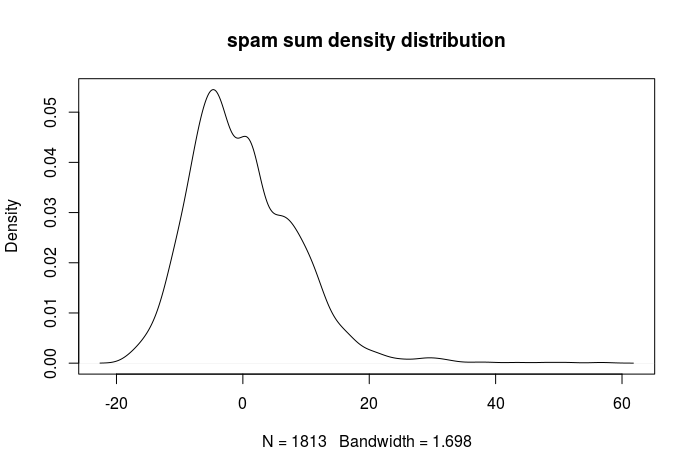
\includegraphics[width=1\textwidth]{img/spamSumDistribution.png}
		\label{f1}
	\end{minipage}
	\hspace{0.1cm}
	\begin{minipage}[t]{0.5\linewidth} 
		\centering
		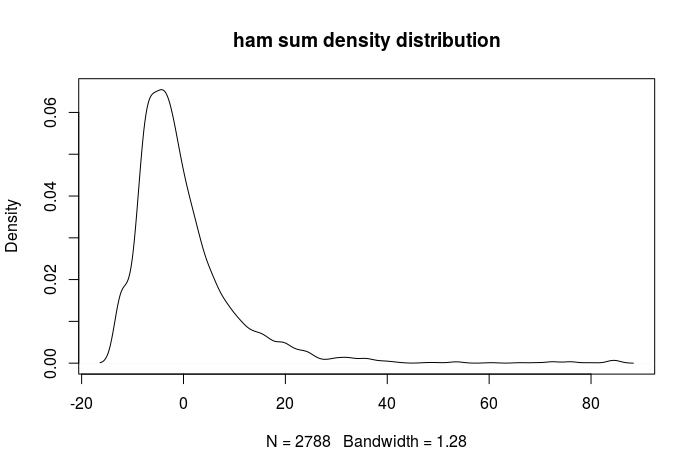
\includegraphics[width=1\textwidth]{img/hamSumDistribution.png}
		\label{f2}
	\end{minipage}        
\end{figure}
From the two density plots it is possible to see that normality is not reached by the sum distribution of both the classes, and also \textit{mardia univariate normality test} returns a very small p-values meaning that the resulting distribution is statistically distant from a normal distribution.

\paragraph{Model parameters}Essentially the main goal of an Naive Bayes classifier is assign the label $y$ which maximize the quantity $p(y|x)$, considering class probability, prior probability and Bayes's Theorem. In order to give some parameter about the generated classifier I decided to split the dataset: $70\%$ for training and $30\%$ for learning. The following results and parameters will consider this composition.

$$
p(spam) = 0.386956
$$
$$ 
p(ham) = 0.613043
$$
\newline
Mean value for each feature with class spam: $\mu_1$:
\begin{table}[!htbp]
	\begin{tabularx}{\linewidth}{|l|l|l|l|l|l|l|}
	\cline{1-7}
	\centering 1.570e-01 & 1.670e-01 & 4.100e-01 & 1.770e-01 & 4.980e-01 & 1.740e-01 & 2.760e-01\\
	\cline{1-7}
	\centering 2.010e-01 & 1.670e-01 & 3.600e-01 & 1.170e-01 & 5.440e-01 & 1.530e-01 & 8.700e-02\\
	\cline{1-7}
	\centering 1.190e-01 & 5.040e-01 & 2.760e-01 & 3.110e-01 & 2.252e+00 & 1.930e-01 & 1.355e+00\\
	\cline{1-7}
	\centering 2.200e-01 & 2.660e-01 & 1.980e-01 & 2.000e-02 & 9.000e-03 & 1.000e-03 & 9.000e-03\\
	\cline{1-7}
	\centering 1.000e-03 & 8.000e-03 & 2.000e-03 & 0.000e+00 & 1.500e-02 & 1.000e-03 & 8.000e-03\\
	\cline{1-7}
	\centering 3.100e-02 & 4.200e-02 & 4.000e-03 & 1.200e-02 & 3.600e-02 & 0.000e+00 & 2.000e-03\\
	\cline{1-7}
	\centering 8.000e-03 & 8.000e-03 & 1.220e-01 & 1.000e-02 & 2.000e-03 & 2.000e-03 & 2.100e-02\\
	\cline{1-7}
	\centering 1.150e-01 & 8.000e-03 & 5.240e-01 & 1.860e-01 & 9.000e-02 & & \\
	\cline{1-7}
		
	\end{tabularx}
\end{table}

\newpage

Variance for each feature with class spam: $\Sigma_1$:

\begin{table}[!htbp]
	\begin{tabularx}{\linewidth}{|l|l|l|l|l|l|l|}
	\cline{1-7}
	\centering 9.000e-02 & 1.080e-01 & 2.430e-01 & 5.675e+00 & 4.810e-01 & 9.600e-02 & 3.250e-01 \\ 
	\cline{1-7}
	\centering 2.400e-01 & 1.240e-01 & 4.260e-01 & 6.100e-02 & 3.770e-01 & 1.420e-01 & 9.300e-02 \\ 
	\cline{1-7}
	\centering 1.650e-01 & 8.190e-01 & 3.390e-01 & 4.030e-01 & 2.371e+00 & 6.400e-01 & 1.388e+00 \\ 
	\cline{1-7}
	\centering 1.784e+00 & 2.960e-01 & 2.740e-01 & 3.400e-02 & 1.000e-02 & 0.000e+00 & 9.000e-03 \\ 
	\cline{1-7}
	\centering 0.000e+00 & 1.500e-02 & 2.000e-03 & 0.000e+00 & 1.300e-02 & 0.000e+00 & 5.000e-03 \\ 
	\cline{1-7}
	\centering 2.300e-02 & 6.100e-02 & 3.000e-03 & 8.000e-03 & 2.100e-02 & 0.000e+00 & 1.000e-03 \\ 
	\cline{1-7}
	\centering 2.000e-03 & 5.000e-03 & 8.400e-02 & 8.000e-03 & 0.000e+00 & 1.000e-03 & 8.000e-03 \\ 
	\cline{1-7}
	\centering 1.050e-01 & 2.000e-03 & 5.840e-01 & 1.420e-01 & 5.170e-01 & & \\
	\cline{1-7}
	\end{tabularx}
\end{table}



Mean value for each feature with class ham: $\mu_0$:

\begin{table}[!htbp]
	\begin{tabularx}{\linewidth}{|l|l|l|l|l|l|l|}
		\cline{1-7}
		\centering 7.500e-02 & 2.610e-01 & 2.010e-01 & 1.000e-03 & 1.770e-01 & 4.100e-02 & 8.000e-03 \\
		\cline{1-7}
		\centering 3.200e-02 & 3.700e-02 & 1.730e-01 & 2.400e-02 & 5.440e-01 & 6.200e-02 & 4.200e-02 \\
		\cline{1-7}
		\centering 8.000e-03 & 6.700e-02 & 4.400e-02 & 1.040e-01 & 1.249e+00 & 7.000e-03 & 4.590e-01 \\
		\cline{1-7}
		\centering 4.700e-02 & 7.000e-03 & 1.100e-02 & 8.490e-01 & 4.240e-01 & 1.329e+00 & 1.820e-01 \\
		\cline{1-7}
		\centering 1.530e-01 & 1.570e-01 & 1.010e-01 & 6.800e-02 & 1.560e-01 & 6.900e-02 & 1.620e-01 \\
		\cline{1-7}
		\centering 1.350e-01 & 2.010e-01 & 1.800e-02 & 1.180e-01 & 7.300e-02 & 8.300e-02 & 2.200e-01 \\
		\cline{1-7}
		\centering 7.600e-02 & 1.160e-01 & 4.090e-01 & 3.060e-01 & 9.000e-03 & 5.400e-02 & 5.100e-02 \\
		\cline{1-7}
		\centering 1.540e-01 & 2.100e-02 & 9.600e-02 & 1.100e-02 & 2.100e-02 & &  \\
		\cline{1-7}
	\end{tabularx}
\end{table}

Variance for each feature with class ham: $\Sigma_0$:

\begin{table}[!htbp]
	\begin{tabularx}{\linewidth}{|l|l|l|l|l|l|}
		\cline{1-6}
		\centering 8.3000e-02 & 2.8780e+00 & 2.6200e-01 & 1.0000e-03 & 3.5700e-01 & 3.5000e-02\\
		\cline{1-6}
		\centering 9.0000e-03 & 4.4000e-02 & 3.0000e-02 & 4.9100e-01 & 2.6000e-02 & 1.0030e+00\\
		\cline{1-6}
		\centering 6.9000e-02 & 1.3000e-01 & 8.0000e-03 & 2.9700e-01 & 3.9000e-02 & 1.7900e-01\\
		\cline{1-6}
		\centering 2.9270e+00 & 9.0000e-03 & 1.1470e+00 & 3.8600e-01 & 6.0000e-03 & 1.1000e-02\\
		\cline{1-6}
		\centering 3.8430e+00 & 1.0560e+00 & 1.9567e+01 & 3.6300e-01 & 5.6800e-01 & 2.9000e-01\\
		\cline{1-6}
		\centering 2.6100e-01 & 1.4600e-01 & 5.4300e-01 & 1.4600e-01 & 4.7600e-01 & 2.3100e-01\\
		\cline{1-6}
		\centering 2.5500e-01 & 7.1000e-02 & 2.7500e-01 & 1.5100e-01 & 2.6000e-01 & 9.7700e-01\\
		\cline{1-6}
		\centering 9.5000e-02 & 5.6200e-01 & 1.6930e+00 & 1.5510e+00 & 1.0000e-02 & 1.5500e-01\\
		\cline{1-6}
		\centering 9.1000e-02 & 5.8000e-02 & 1.4000e-02 & 3.3900e-01 & 3.0000e-03 & 5.6000e-02\\
		\cline{1-6}
	\end{tabularx}
\end{table}

\newpage
\section{Comparison}
The request for this assignment is to compare two types of classifiers, SVM and Naive Bayes, building a spam filter given a dataset which already represents spam/ham email through a bag-of-words representations. The main goal of each classifier is to find a function that given a message return $1$ if the message is considered as spam or $0$ otherwise. During the report we have seen that the two approaches belong to two specific families of classifiers, in particular SVM can be considered as a discriminative classifiers and Naive Bayes can be considered as a generative one.
\textbf{Discriminative classifiers} focus on learning a decision boundary $h(x)$ which separates as better as possible the considered class, in our case spam/ham. The role of this \textbf{decision boundary} (function) is to discriminate between different classes. They allow you to classify points, without providing a model of how the points are actually generated or how features are related to the correspondent class.\\
\textbf{Generative} classifiers focus on learning the underlying data distribution, in particular try to learn the \textbf{join probability} $p(x,y)$ directly from data taking advantage of some possible assumptions. Both the two strategies are adopted depending on the dealing problem, since each of them has particular advantages and disadvantages that should be considered.\\
The following pictures give an idea on how the two approaches manage the input problem and how they take their final decision in order to classify data points from a geometric point of view:

\begin{figure}[!h]
	\begin{minipage}[t]{0.5\linewidth}
		\centering
		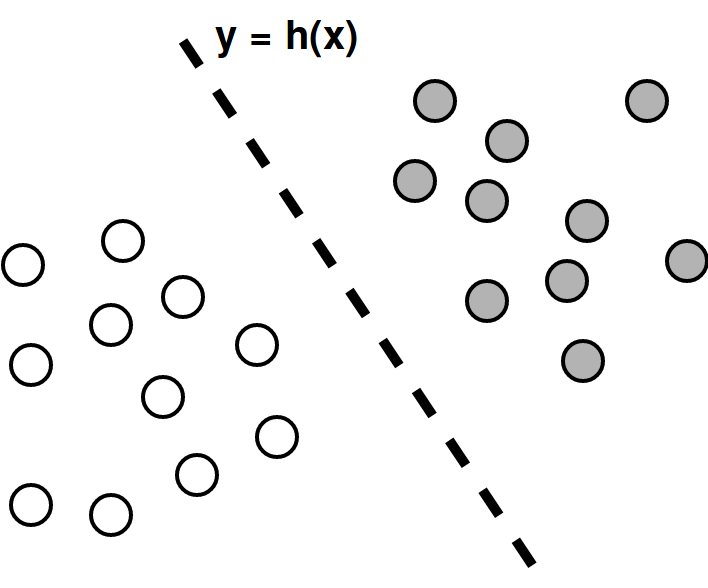
\includegraphics[width=0.60\textwidth]{img/discriminative_geometry2.png}
		\caption{Discriminative models}
		\label{f1}
	\end{minipage}
	\hspace{0.1cm}
	\begin{minipage}[t]{0.5\linewidth} 
		\centering
		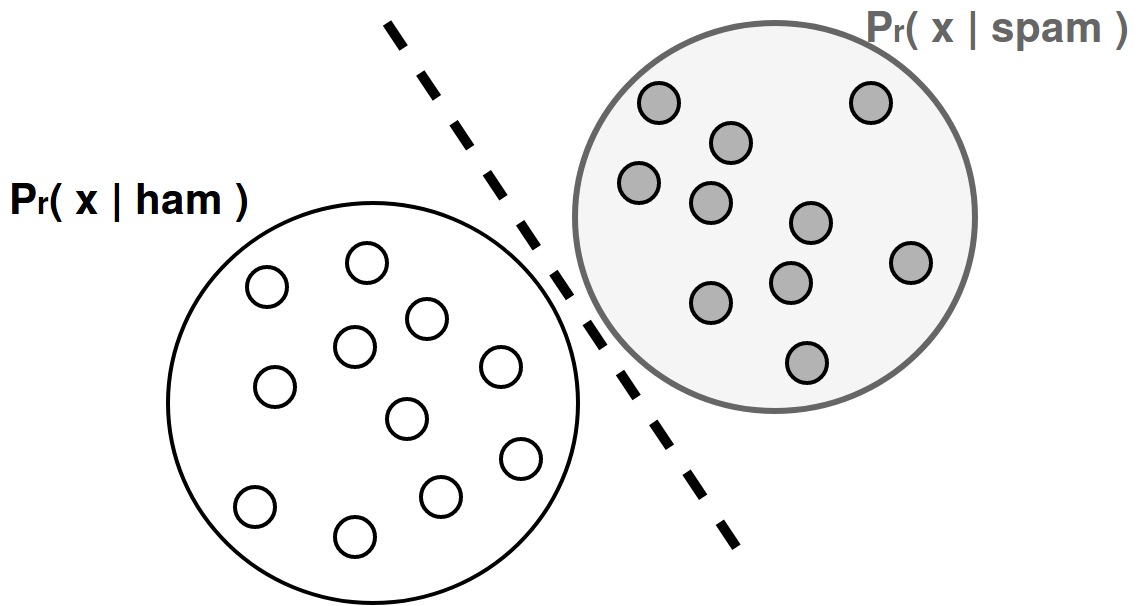
\includegraphics[width=0.9\textwidth]{img/generative_geometry2.png}
		\caption{Generative models}
		\label{f2}
	\end{minipage}        
\end{figure} 
As we can see in general the role of a generative classifier is more difficult, it is not limited on learning a function but probability distributions, and for this reason it requires some non simple assumptions. For sure one advantage of generative approaches is that knowing the joint probability distribution $p(x,y)$ it is possible to generate new possible pairs $(x,y)$. Another advantage of generative classifiers is that with them it is possible to identify possible outliers. 

\image{img/outlier2.png}{Outliers}{0.45}
We can see from the previous image that the red point is basically a possible outlier, respect to the training data. Considering for instance SVM with $h(x)$ as decision function, we know that the greater is the distance from the decision boundary the greater is the affability of the resulting classification. So we can have two cases: that point is simply affected by noise and it is correctly classified, or it is a point generated from another different distribution for which the class probability is lower but it exists. For the first case both the two model will classify correctly the point, but with Naive Bayes we can observe that both the two probability $p(x | spam)$ and $p(x | ham)$ are very small and this can be an evident signal of the presence of another possible distribution. In this way it is possible to discover possible \textbf{underlying distributions}.

Another interesting point of comparison is the time required for learning phase in fact SVM, even if it considers only support vectors and not all the data points, requires more iterations to find the right parameters in order to find the best hyperplane. Instead the training phase of Naive Bayes classifier requires less data and it is very simple since it is performed with a single iteration.
Until now we have seen the strength of Naive Bayes classifier, and in general of generative classifiers, but main point is that there two fundamental assumptions: \textbf{conditionally independence} between variables and \textbf{normal probability distribution}. These two assumptions are not always completely satisfied in the real words, as we have seen during this assignment.\\
If the Naive Bayes assumptions are not satisfied, discriminative classifiers tend to outperform Naive Bayes classifier as the size of the dataset increase. This result is given by the fact that dependency structure cannot be captured by the Naive Bayes classifier, instead discriminative classifiers are not affected by this structure and when the dataset increase the performance improve. Of course it can happen that with small data set discriminative models might consider false patterns, remember that data are influenced by the presence of noise. In practice, discriminative classifiers could be better than generative classifiers in presence of a large set of data that does not preserve the required assumptions. In general a generative classifier works well and learn the underlying structure of the data if the model is right specified and assumptions are satisfied.

\section{Conclusion}
During this assignment we have played with two different types of classifiers: Support Vector Machine and Naive Bayes. In the comparison section we have analyzed the main differences between the two models, considering advantages, disadvantages and case of application for both. Some conclusion can be considered at the end of this assignment. Starting from SVM we have seen its very powerful framework to deal with non linearly separable data, through the usage of \textbf{kernel trick}. The idea of transforming the original feature space into another one, with same number of dimension or higher, can change completely the prediction capacity of our classifier. In particular we have seen 3 types of kernels: linear, polynomial and radial basis function. Another particular aspect of SVM is the consideration of length of the input vectors. Since SVM can be written in terms of dot product we know that this operator is affected by length, and in same cases we are not interested on the length evaluation but only on the vector direction (angular information). For this reason a new analysis was done, considering new kernels that apply the normalization of the input vectors, such that at the end all the vectors have length = 1. The results obtained with these new kernels in general are better the the original one, and this can be reasonable since in most application which involve text similarity (like recommender system) use as similarity measure direction of vectors instead of their length.\\
The second approach provided Naive Bayes classifier does not give better results respect to angular kernels used in SVM. We have seen that the main reason is probably the fact that Naive Bayes assumption are not satisfied and this does not allow the algorithm to learn particular patterns but instead we the increase of data it is not able to capture some information.  

\end{document}
